\documentclass[a4paper,10pt,twocolumn]{article}
\usepackage[utf8]{inputenc}

%opening
\title{Filesystem for Job Submission to Grid System}
\author{Josef Kejzlar}

%packages
\usepackage{graphicx}
\usepackage[pdfauthor={Josef Kejzlar},
pdftitle={Filesystem for Job Submission to Grid System},
bookmarks=true,
colorlinks=true,
breaklinks=true,
urlcolor=red,
citecolor=blue,
linkcolor=blue,
unicode=true]{hyperref}
\usepackage[square, numbers]{natbib}

\newcommand{\term}[1]{``#1''}
\newcommand{\code}[1]{\textit{#1}}

\begin{document}

\maketitle

\begin{abstract}
Submitting job to grid system is not an easy task and because there are many different grid software in use, it is hard to find some universal way of submitting user job. Therefore this project tries to introduce user friendly and standardized way of submitting jobs to different grid system using virtual filesystem that acts as a gateway for user. We are trying to minimize necessary user knowledge by exploiting existing Unix standard way of work with virtual filesystem.
\end{abstract}



\section{Introduction}

Submitting a job to grid system is always a little bit tricky, because our executable code and data are transfered to remote location, there run whenever scheduler decides and we have practically no direct control over the process. Yet it is necessary to do some computation in grid system and we have to deal with all obstacles connected with job submission and control.

\subsection{Grid - a wild beast}
Grid system is not something that every researcher can afford to create in his laboratory and these systems are commonly run and administered by IT stuff and not by researches themselves. Therefore there is usually one or two grids available to researcher and he has no way to choose which grid software he will have to deal with. And even though all grid softwares offers some basic common features it is always researcher that has to cope with given grid software feature set and has to adapt program he want to run to the work flow and possibilities of given grid. 

Diversity of grid softwares and necessity to learn new ways of dealing with basic tasks leads to an effort for standardization and unification of access methods to grid system. One result of this effort are libraries trying to offer universal way of accessing grid resources, transparently dealing with differences between grid softwares. Another very common way are standardized interfaces offered directly by grid softwares that can be universally used. Both of these techniques can unfortunately provide access only to the lowest common denominator of features offered by all grid softwares.

Researcher is therefore facing decision whether to fully exploit special features offered by one grid software and be bond to use only this software or to use some generic standardized way and be free to migrate between grids or even use more grids together. We have given ourselves the same question and decided that easy migration, unification and ultimate chance to submit one job to more than one grid is the right way to go. Even though an additional effort is necessary to bend submitted job and submitters work flow to comply with reduced feature set of unified interface.


\subsection{User-friendliness and low barriers}
We would like to bring generic approaches of job submission one step closer to user. It still needs a lot of programming skills to use either generic libraries or unified APIs and there are many caveats caused by complexity of setting up these solutions. We decided to use filesystem as a base interface. Filesystem is one of the best known interfaces that every user has to deal with on daily basis and that proved its quality given the time already in use. Barrier for working with filesystem way of job submission is very low and does not require neither special skills nor special support in tools used by user. Basic file operations can be done in every programming or scripting language and it is possible to do file manipulation even from graphical user interface.

\begin{figure}[t]
 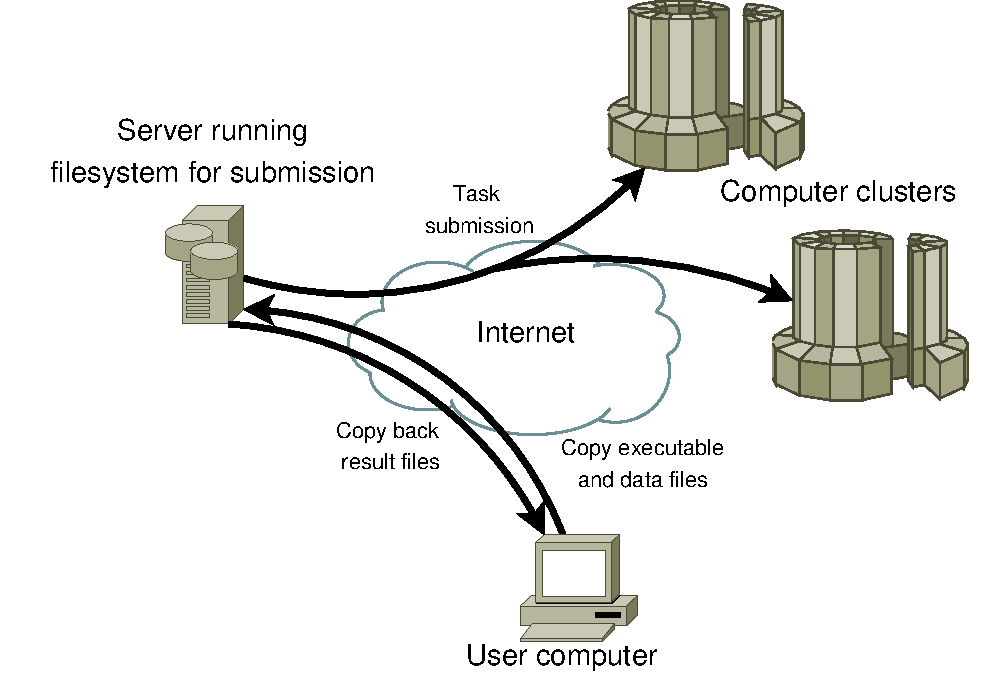
\includegraphics[keepaspectratio=true,width=0.5\textwidth,height=0.5\textheight]{./images/basic_structure.pdf}
 % basic_structure.pdf: 477x328 pixel, 72dpi, 16.83x11.57 cm, bb=0 0 477 328
 \caption{Client submitting job using filesystem to multiple grid systems}
 \label{basic_structure}
\end{figure}


Our basic idea is described by figure \ref{basic_structure}. User copy all the job files to virtual filesystem and than tell filesystem to submit his job to grid. In background software communicate with remote grid system and submit job. User is then notified by filesystem that his job has finished and all the results generated during job's life are available again in filesystem. Whole process should be as easy as possible while retaining good configuration and customization of job submission. 

We also does not want to bond one filesystem instance to one grid and therefore we use term \term{service} that represents connection to concrete grid system. Services are configured by administrators and user can choose during job submission which service he wants to use. This way is user completely shielded from problems with grid communication and does not even have to know what grid software he is submitting job to.



\section{Overview}

This section describes what possibilities filesystem offer to user and how the typical job suitable for submission using filesystem should look like.

\subsection{Condor is our inspiration}
While designing how filesystem interface should look like we had to define work flows that we are going to support natively and that would cover with slight modifications as many existing real world scenarios as possible. We did not want to reinvent the wheel because familiarity with interface lower barrier for acceptance of our solution. Therefore we chose Condor\cite{condor} grid software as a reference software to support, because Condor, given its long history, could be defined as a base for most of other grid software in use. We also use Condor way of submitting \term{cluster job}. Cluster job contains more instances of program able to be running on multiple nodes in parallel and therefore cluster jobs are also called \term{parallel jobs}. In practice most jobs are cluster jobs, because to fully utilize computing power of grid the job has to run on multiple nodes simultaneously.

\subsection{Typical job}
Typical job suitable for submission using our filesystem has executable that can be run in one or multiple instances. User can define input file, that is passed as standard input. Every instance then produces output file and error file where data from standard output and error streams respectively are stored. Executable can also access other files selected by user during submission that can be modified and will be accessible to user after job finishes. User can also customize executable arguments and environment in which the job is launched.

\subsection{Job parameters}
Each job has several parameters that allows customization of submission. First group of parameters is bond to job executable and specify all the values mentioned above - executable file, input file, output file, error file, command-line arguments and environment variables. Second group of parameters is related to grid system. The most important parameter selects which service to use. Other parameters further customize how executable is going to be run - number of processes in cluster job, memory required by job and so on.

\subsection{Cluster jobs}
To support cluster jobs, filesystem interface has to provide some way how to distinguish instances from each other, because usually each instance need to process different data or do slightly different work. Therefore all executable parameters can contain special string \code{\textdollar(process)} that will be replaced by null based instance index. Using this technique, user can define different input/output/error file for each instance. It is also possible to place instance index into executable arguments or in environment variable. So for example user can define input file name as \code{input\_\textdollar(process).txt} and first instance will get file \code{input\_0.txt} passed in, second \code{input\_1.txt}, third \code{input\_2.txt} and so on. This technique of dealing with different parameters for each instance is very efficient because user does not have to specify unique value for every instance and still has good control over parameter value.



\section{Design}

In this section we discuss how we use files and directories to represent submitted job and how we allow user to interact with filesystem.

\subsection{Virtual filesystem basics}
While designing the filesystem way of submitting job we heavily reused techniques from other virtual filesystems commonly in use. Directories represents some logical objects and creates hierarchical tree structure. Files placed in directories allow read and/or write access to properties of these objects and they are very often created automatically and prefilled with default values, so that user always know what properties object supports and what values these properties holds. By simple reading values from files it is possible to get current value of property and by writing into file the property value is set. Symbolic links are also used to represent relations between objects or properties.


\subsection{Our filesystem structure}

\begin{figure}
 \centering
 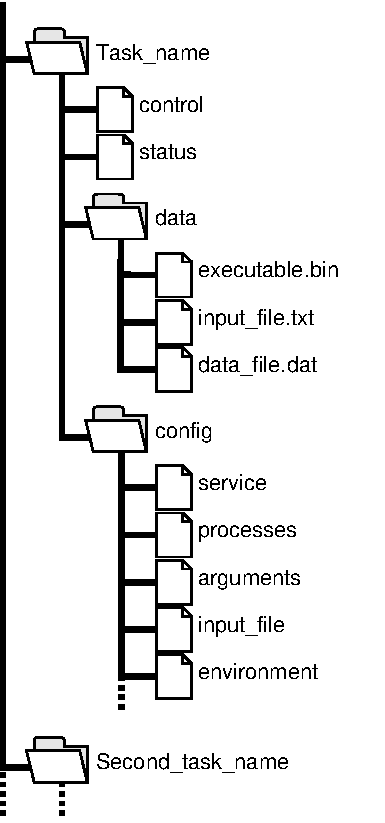
\includegraphics[keepaspectratio=true,width=0.4\textwidth,height=0.4\textheight]{./images/filesystem_structure.pdf}
 % filesystem_structure.pdf: 0x0 pixel, 300dpi, 0.00x0.00 cm, bb=
 \caption{Filesystem structure of job ready to be submitted}
 \label{structure}
\end{figure}

\begin{figure}
 \centering
 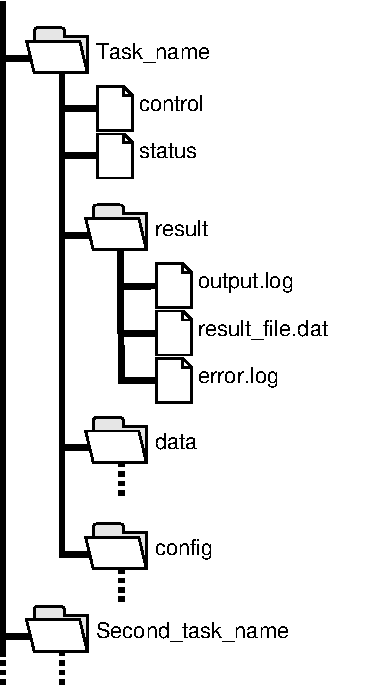
\includegraphics[keepaspectratio=true,width=0.4\textwidth,height=0.4\textheight]{./images/filesystem_structure_after.pdf}
 % filesystem_structure.pdf: 0x0 pixel, 300dpi, 0.00x0.00 cm, bb=
 \caption{Filesystem structure of finished job}
 \label{structure_after}
\end{figure}

\code{Job} itself is the main object we need to work with. Therefore top-level directories of our filesystem represent jobs and user can create new job by simply creating new directory. Job directory serves as a storage for all necessary files to job submission and its name uniquely identifies job and specify job's name. Every job directory automatically contains some subdirectories and files. In \code{config} subdirectory one can find files representing all configuration parameters. User can modify these files to customize job parameters and each parameter has configurable default value. These values specify for example number of processes, name of executable file, name of input file and so on. Another important subdirectory is \code{data} directory where all user-supplied files are stored. User has to copy at least executable file into data directory and of course all the supplementary files required during job execution should be placed there as well. Last directory is \code{result} directory that holds all the files returned from job execution and is automatically created when job finishes. Result subdirectory is the place where user finds all the created or modified data files as well as error and output files produced during job execution.

Each job directory also contains \term{control} file that allows user to issue commands related to job execution. Control file does not ``remember'' any value and always contains all available commands supported by control file. User can write command into control file and this way trigger action represented by command. Typical example of command is \code{start}, \code{abort} or \code{start\_and\_wait}. For example writing \code{start\_and\_wait} into control file cause current job to be executed and writing does not complete until job finishes. If issued command does not complete successfully, writing returns error. This way we can very easily support waiting for some event without need for polling of status in endless loop and we also handle error state in consistent way. Because querying job status is often necessary, there is also \code{status} file inside job directory. Status file is read only and contains numerical and string representation of job current status.

\subsection{Typical work-flow}
As we already mentioned it is very easy to create new job. User just creates new top-level directory and names it. Immediately after creation job directory already contains all the files and directories mentioned in previous paragraphs as can be seen on figure \ref{structure}. Naturally \code{data} directory is initially empty and user is supposed to populate data directory with executable binary and other necessary files. User can also modify files inside \code{config} directory to set job parameters. When job is ready to be submitted command \code{start} or \code{start\_and\_wait} can be written into \code{control} file to initiate job submission. Commands \code{start\_and\_wait} and \code{wait} has special behavior that writing command into file does not exit until job execution finishes or returns error. After job completion user can find all the files generated during jobs life in created \code{result} directory. As can be seen on figure \ref{structure_after}, \code{result} directory is populated with output files, error files where all the errors are logged and other files created by executable. User can copy files from \code{result} directory for additional processing. When user is done with job results he can either destroy job or restart it. For restarting job serves \code{restart} command that deletes all the result files and prepares job for another submission. If user wants to destroy the job he just deletes job folder and all the resources held by job are released.

\subsection{Example of job submission}

Figure \ref{example} shows example how to submit job directly from UNIX shell. User does not need any special tools. The only commands necessary are \code{echo} to modify parameters and send command, \code{cat} to read content of files and \code{cp} to copy files into \code{data} and from \code{result} folders.
Example creates cluster job called \code{test} and submits it to  service \code{Condor}. Job has two processes and as a testing executable is used \code{/bin/cp}. \code{Cp} will receive arguments to copy data file \code{fileIn} to file \code{fileOut}. However we are submitting cluster job so that each instance has to produce unique files and therefore we append \code{\textdollar(process)} to target file of copy operation. This way process 1 will copy \code{fileIn} to \code{fileOut\_0} and process 2 will copy \code{fileIn} to \code{fileOut\_1}.

\begin{figure*}
  \begin{verbatim}
# Current directory is root directory of filesystem

# Creating job 'test'
mkdir ./test

# Using Condor service ...
echo "Condor" > ./test/config/service

# Job status:
cat ./test/status
# output: 0	new

# Copying /bin/cp as binary executable
cp /bin/cp ./test/data/executable

# Creating data file 'fileIn' with some content
echo "sample data file" > ./test/data/fileIn

# Setting argument to '-v fileIn fileOut_$(process)' - copy verbosely file 'fileIn'
echo '-v fileIn fileOut_$(process)' > ./test/config/arguments

# Setting output file to '$(process)'
echo 'output_$(process)' > ./test/config/output_file

# Setting to use 2 processes - cluster job
echo '2' > ./test/config/processes

# Submitting job ...
echo start > ./test/control

# Job status:
cat ./test/status
# output: 2	running

# Waiting for job completion ....
echo wait > ./test/control

# Job status:
cat ./test/status
# output: 5	finished

# Content of result folder:
ls ./test/result
# output: error  fileIn  fileOut_0  fileOut_2  output_0  output_1

# Deleting job 'test'
rmdir ./test
  \end{verbatim}
  \caption{Example of shell session doing job submission}
  \label{example}
\end{figure*}


\section{Implementation}

Here we present implementation details that could be handy for advanced user to understand all possibilities of filesystem interface.

\subsection{Commands}

TODO: Describe all commands available

\subsection{Statuses}

Figure \ref{statuses} describes all possible job states and reasons for job being transfered to each state. Job state can be obtained from \code{status} file in job directory. This file contains number of current state followed by \code{tab} and name of state.

\begin{figure}[h]
  \begin{description}
   \item[0 - new] initial state after job is created. Only in this state it is possible to start job
   \item[1 - submitted] job is submitted and waiting to be scheduled by grid
   \item[2 - running] job is currently running on grid node(s)
   \item[3 - aborted] after calling \code{abort} command
   \item[4 - failed] when job submission to grid failed. Error details are in \code{error} file in \code{result} folder
   \item[5 - finished] when job successfully finished its execution.
   \item[6 - suspended] after calling \code{suspend} command or when grid is not currently able to run the job, possible because of error during execution.
  \end{description}
  \caption{Description of job statuses}
  \label{statuses}
\end{figure}



\section{Limitations and further work}

Here we discuss difficulties that user can face and problems still waiting for proper solution. We also suggests some further areas of development.

\subsection{Overwritten files of cluster jobs}
It is up to the user to ensure, that each instance of cluster job writes results to file having unique filename, because during job finishing all the files from all instances are collected in one directory and files having same filename are overwritten in random order. One solution to this problem could be putting files created by each instance to separate directories, but this would pollute result directory with many folders and many files that user wants to be merged would be copied in every directory.

\subsection{Impossible to control single instance of cluster job}

TODO: Perhaps there could be some mechanism to watch/control single instance of parallel job. At least getting status would be great, but SAGA does not support this.

\subsection{Support for interpreted languages}

TODO: User has to use shell script to launch interpreter or specify correctly "shebang`` first line in script.

\subsection{Support for additional grid softwares}

TODO: Not only Condor

\subsection{Unify style of submission with Windows version}

TODO

\bibliographystyle{plainnat}
\bibliography{bibliography}

\end{document}
